\chapter{Towards vehicular cloud services}
\label{cha:vehicular-cloud-services}

% In this chapter, we present two extensions of the traffic offloading work we have introduced and detailed in the previous chapters. Conceptually, offloading spots can be seen as locations where the trajectories of vehicles can be combined into a logical path followed by the data. In the case of the offloading system, the offloading spots temporarily store the data, allowing to pass it asynchronously from one vehicle to another.

% Talk about the placement of offloading spots -> intractable to infer because of unknown origin-destination matrices. Arbitrary placement of the offloading spots to cover the populations and make trips with electric vehicles (\ie less than 150~km away from each other).

In this chapter, we extend the concept of offloading spots according to two distinct directions as a basis for vehicular cloud services. In the first section of this chapter, we exploit the storage capabilities of the offloading spots to design a distributed vehicular cloud-like system to store and share file generated by mobile users. While services like Dropbox\footnote{\url{http://dropbox.com}} and Google Drive\footnote{\url{http://drive.google.com}} have shown their great potential given their popularity, mobile users often face limitations (\eg high cost, low bandwidth, and limited coverage) when accessing such services through wireless networks including cellular 4G LTE or Wi-Fi. In our system, the offloading spots act as repositories where mobile users upload or retrieve files. To increase the likelihood of finding the requested files in a timely fashion, the repositories distribute the user files among the other repositories by using the existing movements of the users between the repositories.  

% The contribution of this work came into the form of a placement algorithm that determines the locations of a target number of repositories for a given user request deadline. The goals of the placement algorithm are twofold: (1) determine locations such that the allocated repositories serve the maximum number of user requests before they expire and (2) connect the repositories together by the movements of the mobile users to create the network used for file distribution. 


In the second section of this chapter, we dematerialize the offloading spots into pre-defined areas where vehicles come in contact frequently and long enough. We use these areas in the context of the virtualization of a large-scale vehicular network with shared vehicular resources (\eg compute, storage, and sensing) sliced into virtual machines. Virtual machines are allocated to multiple service providers, which leverage the movements of the vehicles and their shared resources to deploy large-scale geo-distributed applications (\eg sensing platforms). With these resources available, the services can benefit from a large collection of distributed mobile nodes to collect, process, and aggregate data to perform real-time analytics and make fast operational decisions~\cite{bonomi2012fog}. We investigate the capacity of the contacts in these pre-defined areas in the context of virtual machine migrations that happen as a result of changes in the physical topology or reallocations of the vehicular resources.

In each of these two extensions, we propose an optimized placement of the offloading spots with regard to the requirements of the services. To this end, we leveraged the concepts of the logical view\index{logical view} we introduced with the offloading overlay to represent the movements of the vehicles between the offloading spots. 

Our main contributions in this chapter are:
\begin{itemize}
    
    \item \textbf{Storage and sharing system} (Section~\ref{sec:vehicular-storage-sharing}). We consider a system that relies on a collection of repositories to store and share user files. We propose a placement of the repositories that exploits the movements of vehicles between the repositories to replicate files in the system.
    
    \item \textbf{Vehicle resource virtualization} (Section~\ref{sec:virtual-vehicular-network}). We virtualize the resources of the vehicles to create large-scale virtual vehicular networks. We propose a placement of geographical areas with the required vehicle density to accommodate transfers of virtual machine migrations via vehicle-to-vehicle communications.

\end{itemize}

In the following, we present our vehicular file storage and sharing system in Section~\ref{sec:vehicular-storage-sharing} and our vehicular network virtualization in Section~\ref{sec:virtual-vehicular-network}.

\section{Vehicular file storage and sharing system}
\label{sec:vehicular-storage-sharing}

In this section, we present the design of a cloud-like file storage and sharing system specifically targeting mobile users in urban environments. We use the storage capabilities of the offloading spots to turn them into repositories where users store and retrieve their files. %Content storage and retrieval was also an issue studied in the context of Delay-Tolerant Networking (DTN)~\cite{fall2003delay}. Examples include TierStore~\cite{demmer2008tierstore} which is a Network File System that relies on very low latency links that intermittently connect the repositories. This makes TierStore well suited in the context of DTNs. Ott and Pitk{\"a}nen~\cite{pitkanen2007redundancy,ott2007dtn} proposed a system based on repositories to cache user content, thus decreasing the latency when retrieving a content. However, both of these approaches. 
We study the impact of placement of the storage repositories such that it guarantees the availability and distribution of the files. We evaluate our placement strategy in the context of the public transportation system of buses operating in San Francisco. 

\subsection{Problem statement}

\begin{wrapfigure}[13]{o}[0.7\marginparwidth]{7.2cm}
    \centering
    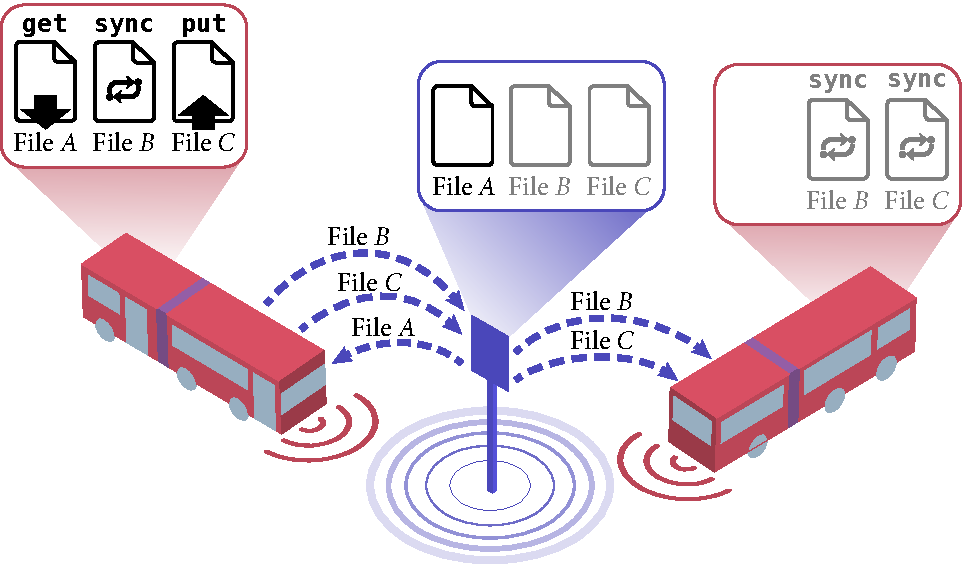
\includegraphics[width=7cm]{figures/message-exchanged.pdf}
    \caption{Requests and data exchanges between a repository and two mobile users when they encounter one another.}
    \label{fig:request-exchange}
\end{wrapfigure}
The system deploys a collection of pre-positioned offloading spots acting as file repositories. They feature high availability, unlimited storage and fast wireless transmission capabilities to handle large data rates in parallel with multiple mobile users. We assume a central controller is in charge of monitoring the files available at each repository. Whenever a repository receives a new file from a user, it notifies the controller of the availability of this file. Likewise, the mobile users can be notified of the availability of the files through the controller. We assume that the communications between the controller and the repositories and mobile users are handled by an inexpensive control channel (\eg SigFox or LoRa)\index{control channel}.

Mobile users with unlimited storage capacity upload or retrieve files to the repositories they encounter as part of their movements. There are two types of user requests: \texttt{put} requests to store user files and \texttt{get} requests to retrieve them. All requests have an associated deadline. Once a mobile user generates a request, the request becomes pending for the user until they encounter a repository. When in the transmission range of the repository, the user seamlessly transfers all of its pending requests to the repository. We assume atomic contacts between the mobile users and the repositories, which allows to transfer an unlimited number of files.

\paragraph{\texttt{put} request.} 
When a mobile user generates a \texttt{put} request, the user waits to be in the transmission range of the first repository it encounters. On an encounter with a repository, the user transfers the \texttt{put} request message along with the file. Once the file is received, the repository updates its local storage and notifies the availability of the file to the central controller. We define the two behaviors of mobile users when they have a \texttt{put} request to execute:
\begin{itemize}

    \item ``First'' \texttt{put} policy: Mobile users immediately delete the request once they transferred it to the first repository they encounter or if its deadline expires, whichever occurs first.

    \item ``All'' \texttt{put} policy: Mobile users delete the request once the deadline associated with the request has expired. This allows the users to potentially replicate the files to all repositories they encounter from the moment the request is generated to the moment it expires.

\end{itemize}

\paragraph{\texttt{get} request.} 
Users share the files they store on the repositories with other users. That is, any user can generate a \texttt{get} request to retrieve any available file. The user then transmits the \texttt{get} request to repositories it meets until the request is satisfied or until its deadline expires, whichever occurs first. In turn, the repository processes the request and transfers the requested file to the mobile user if the file is available in the repository's local storage. Otherwise, the repository notifies the mobile user that the requested file is not available. The mobile user will then try to retrieve the requested file from the next repository it will encounter. If the mobile user does not encounter any repository with a copy of the requested file before the request's deadline expires, the request fails.

The system opportunistically uses the movements of the mobile users to transport the data between the repositories and distribute the files uploaded in the system. Increased file distribution will reduce \texttt{get} failure rates. To accomplish this, we introduce \texttt{sync} requests for the files that need distribution. Repositories generate \texttt{sync} requests once files are stored by their initial uploader, following \texttt{put} requests. A \texttt{sync} request results in transferring copies of a file from the repository to passing mobile users in charge of distributing these copies to repositories along their trajectories. A later encountered repository updates its local storage with the corresponding file and notifies the central controller of the new availability of the file. If the file is yet to be available in every repository, the new repository starts distribution the file it just received by generating corresponding \texttt{sync} requests. Otherwise, the central controller informs the repositories of the distribution completion. 

While replicating files to all the repositories is inefficient in terms of file storage, it fits with our assumption of atomic contacts and unlimited file storage at the users and at the repositories. We further assume no locality bias with respect to where files are generated. Additionally, we assume that we cannot predict the trajectory of the mobile users, in particular, we cannot predict the sequence of storage nodes the mobile users will visit in the future. Under these assumptions, replicating files to all the repositories is the most straightforward approach to increase the availability of files and improve the success ratio of \texttt{get} requests.

The three types of requests \texttt{put}, \texttt{get}, and \texttt{sync} are shown in Figure~\ref{fig:request-exchange}. In this figure, the mobile nodes are buses that aggregate requests from the passengers riding the bus. The first mobile user on the left carries three requests: \texttt{get} for file A, \texttt{sync} for file B, and \texttt{put} for file C. The repository, which only has a local copy of file A, executes all the requests and adds files B and C to its local storage. When a subsequent mobile user encounters the repository, the repository generates \texttt{sync} requests and transfers them to the mobile node, along with the copies of the files. The mobile node then carries the \texttt{sync} requests to the next repository it encounters.


We consider the following metrics to evaluate the performance of our system:
\begin{itemize}

    \item \textbf{Request success ratio.} We aim to maximize the successes and minimize the failures of user requests. A \texttt{put} or \texttt{get} request is successful if it completes before its deadline expires. The success ratio is the number of successful requests divided by the number of all requests issued during the time period of interest. 

    \item \textbf{File distribution duration.} File distribution relies on the movements of the mobile nodes to distribute copies of files across the repositories. The distribution duration of a file is the time it takes for it to be available in all the repositories of the system. The repository placement algorithm takes this metric into account when allocating the location of the repositories to minimize the distribution duration of the files.

\end{itemize}


\subsection{Repository placement}
\label{sec:repo-placement}

The goals of the placement algorithm are twofold: (\textit{i}) determine locations such that the allocated repositories serve the maximum number of user requests before they expire and (\textit{ii}) connect the repositories together by the mobile users' movements to create the file distribution network. The goals of the placement algorithm are represented in Figure~\ref{fig:placement-alg} in the case of a bus transportation system. The bottom layer shows the trajectories of the buses in the  
\begin{wrapfigure}[12]{o}[0.7\marginparwidth]{8.2cm}
    \vspace{-7pt}
    \centering
    \includegraphics[width=7.3cm]{figures/bus-distribution-system.pdf}
    \caption{Different layers to represent the goals of the placement algorithm for a bus transportation system.}
    \label{fig:placement-alg}
%\end{figure}
\end{wrapfigure}
Financial District of San Francisco, with allocated bus stops. Each bus trajectory is represented by a color and a width indicating the frequency of buses. The middle layer shows the discretized demands generated by the bus passengers. This layer shows the demands that are allocated to the repositories placed at the bus stops. Finally, the top layer shows a logical graph where nodes correspond to the allocated repositories and edges to the flows of buses running between two repositories. As in the bottom layer, the width of the edges corresponds to the frequencies of buses. 

We derive the placement of the repositories from a set cover problem, in particular, the Maximal Covering Location Problem~\cite{church1974maximal}. Given a set of candidate locations for the repositories, the placement problem consists in selecting the candidate locations that maximize the success ratio of the requests issued by the users. This problem was shown to be NP-Hard, so we adapt known heuristics to solve it~\cite{megiddo1983maximum}. To this end, we consider the Greedy Adding with Substitution (GAS) heuristic that determines the optimal locations for each iteration of the algorithm~\cite{church1974maximal}. 


\subsubsection{Candidate and demand locations}

The placement algorithm takes both a set $\mathcal{C}$ of candidate locations where the repositories can be placed, as well as a set $\mathcal{D}$ of demand locations to be served by the allocated repositories. The candidate and demands locations refer to geographical places (typically circles and square cells) visited by the user trajectories. The algorithm outputs a set $\mathcal{A}$ of allocated candidate locations for the repositories.

\paragraph{Demands.} 
Users can generate a request at any time. Each successive location visited by the trajectories of the users is a demand location with equal probability of being the starting location of a user request. To this end, we divide the geographical area into a grid of cells of a given size (\eg $100\,\textrm{m}\times 100\,\textrm{m}$). Each cell aggregates the discretized user trajectories that go through the cell. The greater the number of trajectory aggregates, the higher the probability for a cell to be the starting location of user requests.

\paragraph{Candidates.} 
Candidate locations for the repositories correspond to relevant locations the mobile users will often visit for long periods of time, allowing the transfer of significant amounts of data. For instance, candidate locations may be road intersections, or bus stops (\eg in the case of a bus transportation system). In the evaluation section, we use available data from bus transportation systems and consider bus stops as candidates for the location allocation of the repositories.

To determine the locations of the repositories, we quantify the relations between two locations $l_1$ and $l_2$ (either a demand or candidate location) by computing the following spatial statistics:

\begin{itemize}

    \item The mean visit frequency $f(l_1,\,l_2)$ of mobile users that visited location $l_1$, then location $l_2$.

    \item The median inter-visit duration $v(l_1,\,l_2)$ of two consecutive visits of mobile users at location $l_1$ that visited location $l_2$ later in during their trajectory.

    \item The median travel time $t(l_1,\,l_2)$ of the time it takes for a mobile user to travel from location $l_1$ to location $l_2$.

\end{itemize}

We then measure the weight $w(l_1,\,l_2)$ of a pair of locations $(l_1,\,l_2)$ using the visit frequency $f(l_1,\,l_2)$ and the median inter-visit duration $v(l_1,\,l_2)$ as follows:

\begin{equation}
w(l_1,\,l_2) = \frac{f(l_1,\,l_2)}{v(l_1,\,l_2)}\cdot
\end{equation}

In the following, we denote by $\{w_{l_1l_2}\}$  the \textit{weight matrix} such that $w_{l_1l_2} = w(l_1,\,l_2)$, and by $\{t_{l_1l_2}\}$ the \textit{travel time matrix} such that $t_{l_1l_2} = t(l_1,\,l_2)$.


\paragraph{Relations between demands and candidates.} 
The deadline of the user requests imposes a bound $\delta$ on the travel time $t(d,\,c)$ between a demand location $d$ and a candidate location $c$. A demand location $d$ is allocated to a candidate point $c$ if the demand is within the bound $\delta$ and the weight $w_{dc}$ is not null (\ie there are flows of mobile users that travel from the demand to each of the candidates). The goal is to maximize the sum of the weights of the demands $d\in\mathcal{D}$ allocated to a candidate $c$: $\sum_{d\in\mathcal{D}}\{w_{dc}\mid t_{dc} \leq \delta_{dc}\}$. Note that a single demand cell can be allocated to multiple candidates, each within the given bound $\delta$ with non-null weights. 

\paragraph{Relations between pairs of candidates.} 
We characterize the connectivity between two candidates in terms of flows of mobile users travelling from $c_1$ and $c_2$ with both weights $w_{c_1c_2}$ and $w_{c_2c_1}$. For each candidate, we maximize the sum of the weights between this candidate $c$ and the chosen candidates $k\in\mathcal{A}$: $\sum_{k\in\mathcal{A}}w_{kc} + w_{ck}$.


\subsubsection{Location allocation algorithm}

The algorithm derives from greedy-adding with substitution (GAS) heuristic proposed to solve the Maximal Covering Location problem~\cite{church1974maximal}. For each candidate location, we divide the iterations into two parts: selection and substitution. 

\paragraph{Selection.} We first pre-select the set of candidates from the set of remaining candidates such that each candidate is connected to the chosen repositories by the flows of mobile users. This pre-selection is necessary, as it guarantees the creation of the distribution network and increases the availability of files. From these pre-selected candidates, we choose the candidate that maximizes the sum of demand weights within the bound $\delta$ as we defined previously. 

\paragraph{Substitution.} The second part of the algorithm goes back on the previous iterations and examines each allocated candidate and tries to find a better candidate that maximizes the demand weights, while guaranteeing that the new candidate will be connected to the chosen candidates. If a better candidate is found, it replaces the candidate under examination. The substitution part allows to replace the candidates allocated in the early iterations that are not justified in the later iterations due to subsequent allocated candidates.

We adapt the GAS heuristic to our system as follows.  The first candidate is chosen such that it maximizes the sum of demand weights within the bound $\delta$. Note that, since the demand weights are maximized for this candidate, the candidate is often visited by mobile users, making it a good intermediary node to be connected to the other candidates by the flows of mobile users. There is no substitution part, as no other candidate was already chosen. In our implementation, once a candidate is chosen, we remove all the candidates in the vicinity of the chosen candidate (in terms of travel time and distance from the chosen candidate, \eg half the deadline and the distance corresponding to this duration with average speed). This allows us to better spread the repositories over the geographic area and avoids cluttering denser regions with too many repositories.

\subsection{Real experiment simulation}
\label{sec:repo-evaluation}

We run our evaluation in two parts. The first part corresponds to the allocation of a given number of repositories for the given deadline. The second part is the simulation of the system with the repositories placed in the area.

\begin{figure*}[t]
    \begin{subfigure}[b]{0.44\textwidth}
        \centering
        \includegraphics[width=0.9\linewidth]{figures/sf-muni-placement.pdf}
        \caption{Allocation of the repositories. The color variations of the demand and candidate locations represent hotspots resulting from the Getis Ord-G spatial analysis with respect to the bus visit frequencies at these locations~\cite{getis1992analysis}.\vspace*{1.3em}}
        \label{fig:sf-muni-placement}
    \end{subfigure}
    \quad
    \begin{subfigure}[b]{0.54\textwidth}
        \centering
        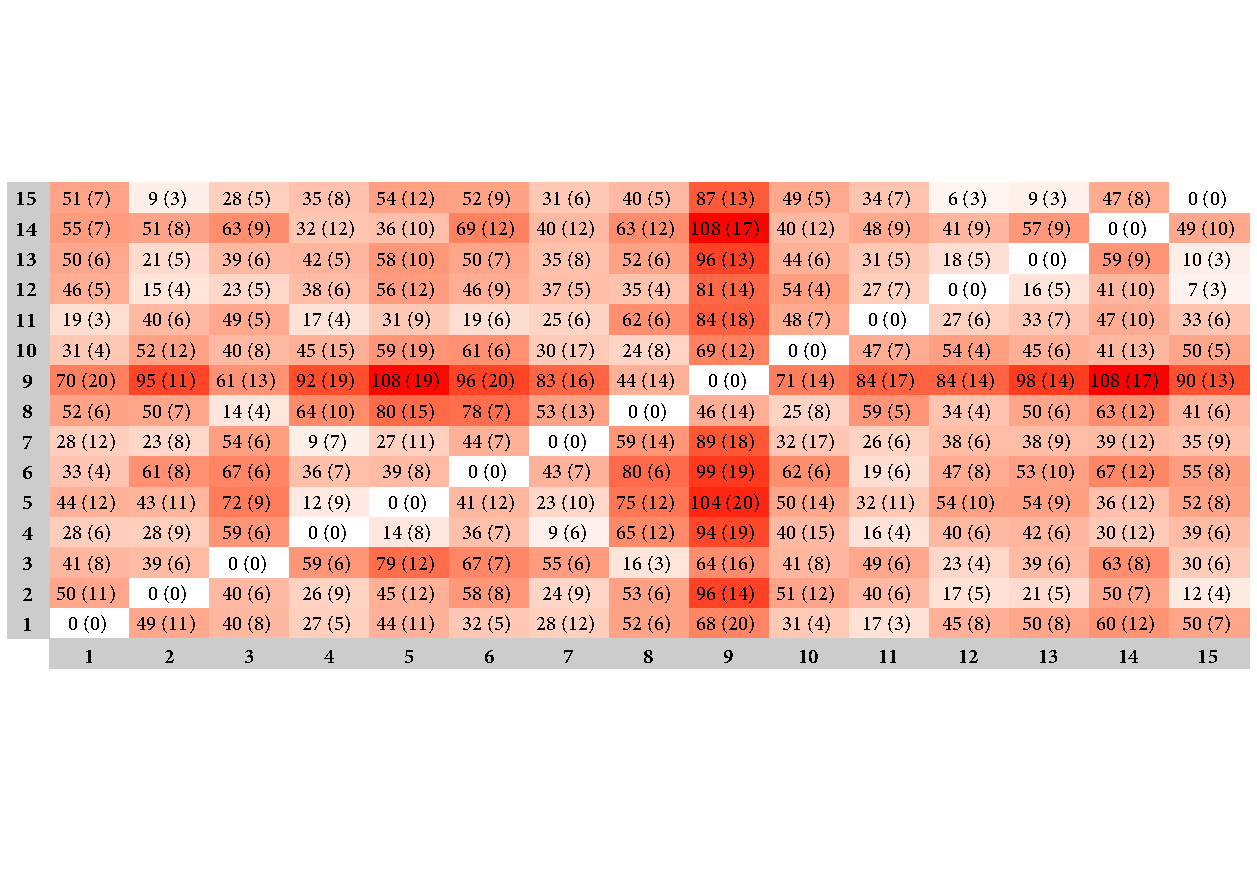
\includegraphics[width=\linewidth]{figures/origin-destination-matrix-1.pdf}
        \caption{Origin-destination matrix of the repositories (identified by the numbers represented on the Figure~\ref{fig:sf-muni-placement} showing the mean travel time in minutes between each pair of repositories. The values in parentheses are the corresponding standard deviation. The simulations were done for 15 repositories placed as shown in Figure~\ref{fig:sf-muni-placement}.}
        \label{fig:propagation-times-matrix}
    \end{subfigure}
    \caption{Results for the allocation of 15 repositories in San Francisco using the bus movements of the MUNI bus transportation system.}
\end{figure*}

\paragraph{Mobility model for public transit vehicles.} Firstly, we simulated the movements of the San Francisco MUNI buses\footnote{\url{https://www.sfmta.com/}} using the ONE simulator~\cite{keranen2009one}. The ONE simulator is a time-discrete and event-based simulator of delay-tolerant networks. We used the \texttt{MapRouteMovement} mobility model implemented in ONE to simulate the movements of mobile nodes and their stops on a street map. This mobility model is particularly well suited to simulate the movement of buses that are part of a transit system. We derive the movements of the buses from GTFS (\textit{General Transit Feed Specification})\footnote{\url{https://developers.google.com/transit/gtfs}} feeds given by the MUNI transit authority that gather the buses' schedules. We develop generic tools to convert the GTFS feeds into a collection of \texttt{MapRouteMovement} mobility models compatible with the ONE format.

\paragraph{Repository placement.} Secondly, we developed a framework to determine the locations of the repositories. The framework implements the algorithm described in Section~\ref{sec:sf-muni-placement}. It takes the bus movements we derived from the GTFS feeds. We divide the geographical area into a grid of cells of size 100m~$\times$~100m. We take bus stops as candidates to host a repository, since the buses stop for a long enough duration to transfer large amounts of data. The framework then allocates the locations of the target number of repositories among the candidate locations, given user request deadline. We represented in Figure~\ref{fig:sf-muni-placement} the output allocation of 15 repositories' locations out of the 4,590 bus stops in San Francisco using the movements of the MUNI buses. In this figure, we show a Getis Ord-G hotspot analysis of the spatially significant bus stop candidates with regards to the visit frequencies of the buses in their vicinity~\cite{getis1992analysis}.


%We simulate the bus movements of the San Francisco MUNI transit system.\footnote{\url{https://www.sfmta.com/}} 
After running our methodology to convert the GTFS feed, we obtained the movements of 493 buses running on 130 different trajectories, which represents the traffic of buses running between 10am and 4pm on a typical weekday. Both the mobile users and the repositories are equipped with WiFi network interfaces with a range of 250~m. We ignore wireless interference and assume enough wireless capacity to accommodate the full exchange of files between the repositories and the mobile users. The candidate locations are the bus stops given by the GTFS bus feed projected onto the street map. The wait time of the buses at the bus stops is picked at random between 10~seconds and 30~seconds. The mobile users send requests independently every 10~minutes following a Poisson distribution, without any assumptions on the popularity and geographical locality of the files. We assume the mobile users generate the \texttt{put} and \texttt{get} requests as follows: 10\% of the requests are \texttt{put} requests and 90\% of the requests are \texttt{get} requests. We assume the mobile users generate the \texttt{put} and \texttt{get} requests. The simulation duration is 20,000~seconds. For each simulation, we deploy a target number of repositories up until the optimal number of repositories, where no demands are left unallocated. 

\begin{figure}[t]
    \centering
    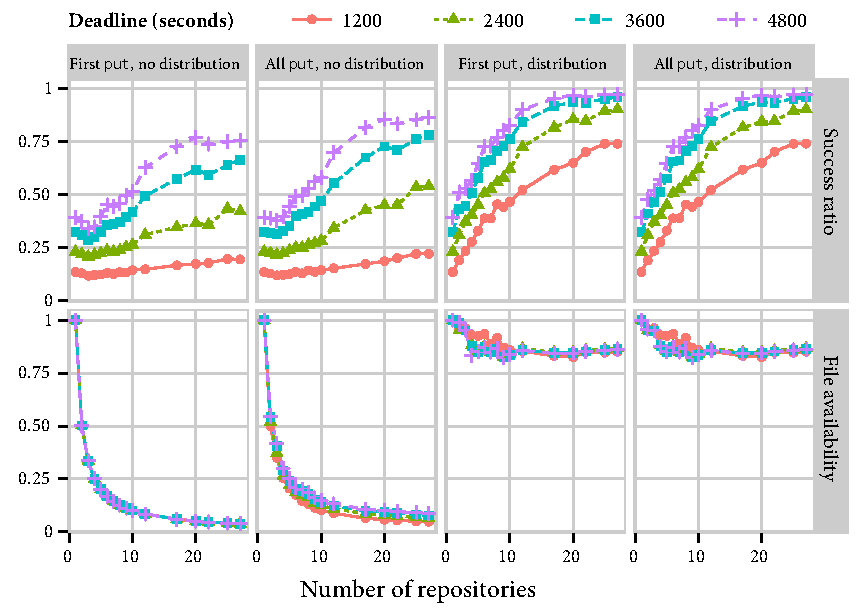
\includegraphics[width=0.8\linewidth]{figures/successRatio-fileAvailability.pdf}
    \caption{Comparison of the impact of the different \texttt{put} policies and the existence of the distribution network in the user request success ratio and the file availability in the repositories.}
    \label{fig:baseline1}
    % ggplot(r, aes(x=V3,colour=as.factor(V2), shape=as.factor(V2), linetype=as.factor(V2), y=V11)) + geom_line() + geom_point() + xlab("Number of repositories") + ylab("Success ratio of user requests") + scale_colour_manual(values=c("#f8766d","#00ba38","#619cff", "purple"), name="Deadline (s)")+ scale_linetype_discrete("Deadline (s)") + scale_shape_discrete("Deadline (s)") + facet_grid( ~ V1)
\end{figure}

\paragraph{Success ratio.} 
As a first step, we perform the simulations to evaluate the benefits of the \texttt{put} policies and the distribution network in the success ratio of the user requests. To this end, we simulate the system under different assumptions regarding the \texttt{put} policy (``first''  or ``all'') and the existence of the distribution network. We represent the average success ratio of the \texttt{get} user requests and the file availability in the repositories in Figure~\ref{fig:baseline1}. In the scenario with the ``first'' \texttt{put} policy and no distribution network, we notice that the more repositories there are, the more user requests are satisfied. Some buses that have pending \texttt{get} requests are not able to reach any repository because of their routes and the few repositories available. Adding more repositories allows more buses to reach repositories, resulting in better success ratio of the \texttt{get} user requests. However, since the data is scattered across multiple repositories, the success ratio of the \texttt{get} requests still remains low for short deadlines. For long deadlines, the buses visit more repositories, which increases their chances to visit one with a copy of the requested file. Taking advantage of the ``all'' \texttt{put} policy helps to increase the success ratio of the \texttt{get} requests by 9.98\% on average for all the deadlines. With this policy, the buses distribute copies of the files to different repositories, thus increasing the availability of the files. Contrary to the ``first'' \texttt{put} policy where user files are available at only one repository, the ``all'' \texttt{put} policy increases the chance of a mobile user to find a repository with a local copy of the requested file.

The distribution network led to increase the user request success ratio by 104.3\%. Note that this improvement is greater for lower user request deadlines (\eg the improvement for the user requests of 1200~seconds is of 201.4\% on average). The distribution network distributes copies of the files in several repositories. Since the repository placement algorithm guarantees that all the repositories are connected together, the files can be distributed to each repository of the system. Hence, a mobile user with a pending \texttt{get} request is more likely to encounter a repository that has a local copy of the requested file, which increases the success ratio of the \texttt{get} requests. Note that the use of the ``all'' \texttt{put} policy does not change anything in the request success ratio and file availability compared to the ``first'' \texttt{put} policy, as the mobile user that originated the request is also part of the distribution network.

\begin{wrapfigure}[14]{o}[0.7\marginparwidth]{8.2cm}
    \vspace{-15pt}
    \centering
    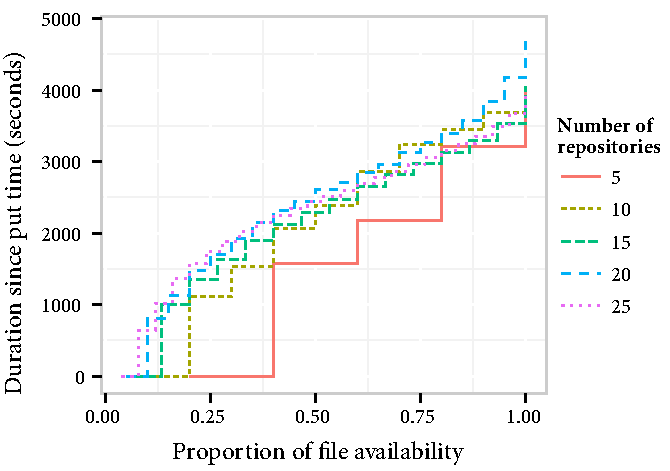
\includegraphics[width=8cm]{figures/propagationTimes.pdf}
    \caption{Distribution duration as a function of the file availability for different numbers of repositories. 
    %and a deadline of 2400~s.
    }
    \label{fig:propagationTimes}
    % ggplot(p, aes(x=V3,colour=as.factor(V1),shape=as.factor(V1), linetype=as.factor(V1),y=V4)) + geom_step() + xlab("Proportion of file availability") + ylab("Duration since put time")
%\end{figure}
\end{wrapfigure}
\paragraph{File availability.} 
We compare the benefits of the distribution network with the ``all''  \texttt{put} policy using the ``File availability'' plots in Figure~\ref{fig:baseline1}. The plots show the proportion of files available in the repositories, where ``1.0'' of file availability corresponds to all the files being available at each repository. We clearly see the benefits of the distribution network to distribute the files among the repositories. The ``all'' \texttt{put} policy also distributes the files to several repositories, however, it fails to distribute the files to repositories beyond those located on the routes of the mobile users that generated the \texttt{put} requests. The plot further shows that, even with the distribution network, the files are not available at every repository (only 85\% of them). In fact, the data represented accounts for the files that were not fully distributed by the end of the simulation. 

\paragraph{Distribution duration.} 
In the second step of our evaluations, we study the distribution duration of the copies of user files among the available repositories. In Figure~\ref{fig:propagationTimes}, we show the average duration to distribute a file throughout the distribution network since the time the file was stored in the first repository (following a \texttt{put} request). We represent the distribution duration of the copies of user files as a function of the proportion of the file availability for different numbers of repositories. For example, with 10 repositories, 40\% of file availability corresponds to the file being available in four repositories. The first repository where the file is stored can be any of the repositories available. We notice that the average time needed to distribute the user files to every repository, regardless of the number of repositories available, is 4000~seconds, or a little more than one hour. It takes more time to distribute the copies of the files to the repositories at the beginning and end of the file distribution. At the beginning of the file distribution, only one copy of the files is available in the first repository. It takes on average 700~seconds to distribute the first copy of the file to the second repository. As more repositories distribute copies of the files, the distribution of the copies becomes faster. By the end of the file distribution, copies of files are available in most repositories. It takes on average 500~seconds to reach the last repository, as it is the farthest away from the first repository where the original copy of the file was stored.

In Figure~\ref{fig:propagation-times-matrix}, we give an origin-destination matrix that shows the average travel time in minutes between any pair of repositories. This translates to the time needed to distribute the file to different repositories from the time the file was stored in a first repository. These values give the average duration for a file to be available at a repository, depending on the originated repository. In the figure, the repositories are identified by the same numbers as the ones in Figure~\ref{fig:sf-muni-placement}. The connectivity between two repositories depends on the number and frequency of the buses going from one repository to another. For instance, repositories 1 and 15 are very well connected to the rest of the repositories. However, repository 9 is not as well connected since it is farther away from the rest of the repositories. This further explains the longer time it takes to distribute copies of the user files from repository 9 to every other repository. This goes to show that the further away the repositories are, the more time it takes on average to reach them and distribute copies of the files to them. 

\clearpage
\section{Virtual machine migration in vehicular networks}
\label{sec:virtual-vehicular-network}

\begin{wrapfigure}[18]{o}[0.7\marginparwidth]{8.2cm}
\centering
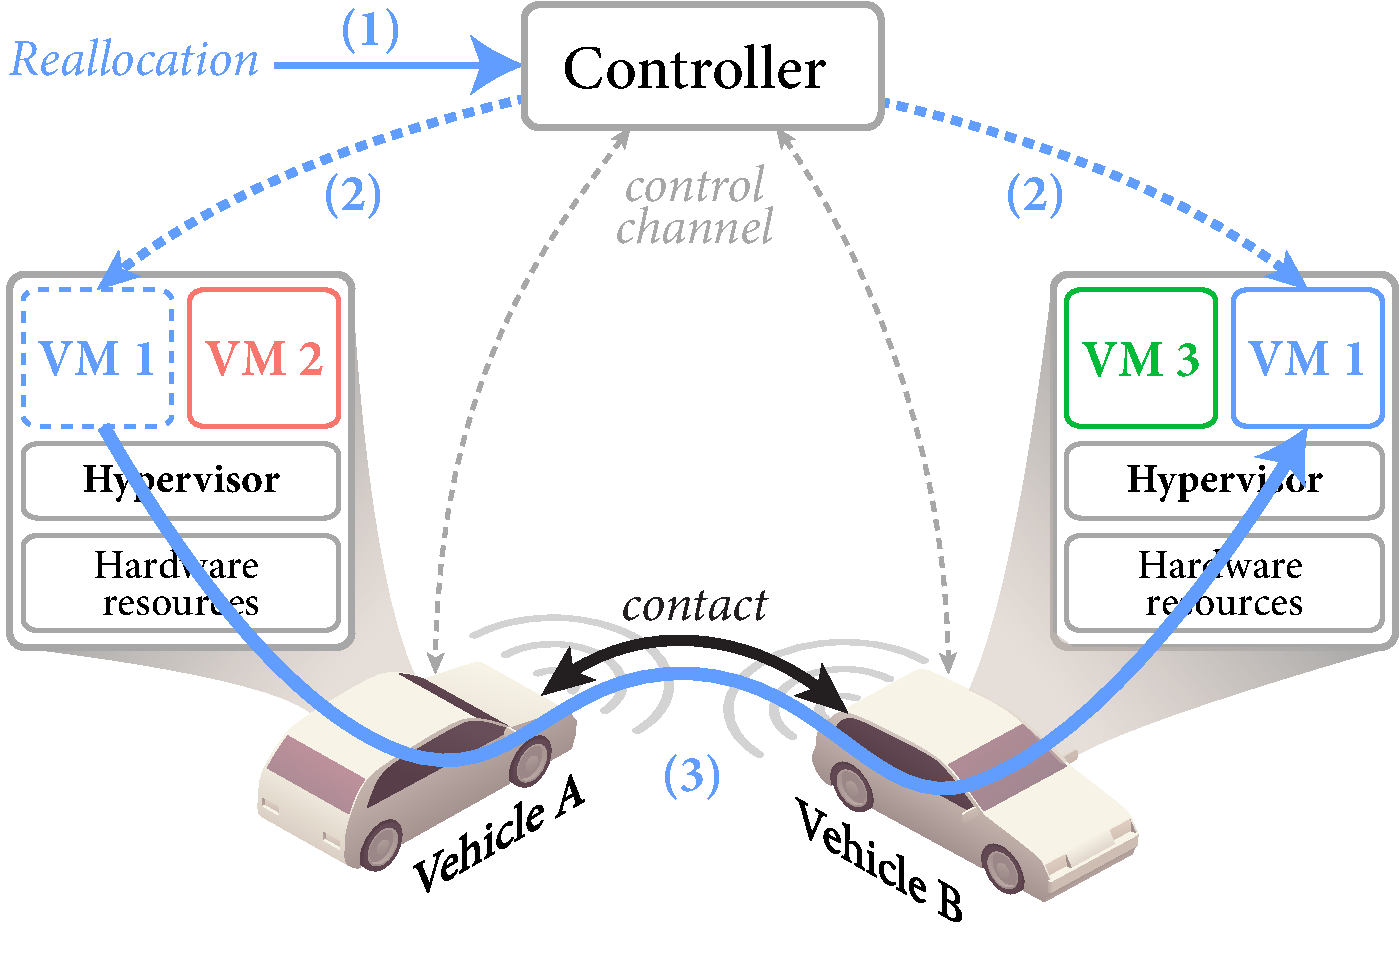
\includegraphics[width=8cm]{figures/VMMigration.pdf}
\caption{Virtual machine migration between two vehicles in contact: \textbf{(1)} The controller receives a reallocation demand of the resources on vehicles A and B: VM 1 has to move from A to B. \textbf{(2)} The controller notifies the two vehicles to initiate the migration during their next contact. \textbf{(3)} When there is a contact, the VM is transferred from A to B.}
\label{fig:vm-migration}
\end{wrapfigure}
In this section, we dematerialize the offloading spots into areas where the vehicles often come in long contacts via \acrfull{v2v} communications\index{contact}. We use these areas in the context of large-scale mobile networks to address the problem of virtualizing the resources of vehicular nodes (\ie compute, storage, and sensing) to create a virtual vehicular network\index{virtual vehicular network}. The vehicular resources are managed by an infrastructure provider through a centralized controller and allocated to service providers who configure the virtual machines to deploy geo-distributed services (\eg large-scale sensing platform). In particular, as shown in Figure~\ref{fig:vm-migration}, we focus on the migration of virtual machines triggered by the re-allocations of virtual resources or changes in the physical topology. Instead of using cellular connectivity, we leverage vehicle-to-vehicle communications to migrate the virtual machines.

This contribution draws on the results presented for various cities including San Francisco and Warsaw where it was shown that vehicles come in contact often and for long period of time in specific areas~\cite{kang2004extracting,sarafijanovic2006island,uppoor2014generation,naboulsi2013instantaneous}. We present a generic methodology for analyzing contact opportunities in urban scenarios where mobility traces are available for various types of vehicles. By limiting the virtual machine migrations to these specific areas, the expected benefit is an improved ratio of successful migrations. We first present this methodology and then evaluate its benefits in the context of virtual machine migrations among the public buses of the city of Dublin, Ireland.


\subsection{Contact density heatmap generation} 

The methodology consists first in processing the mobility traces with the purpose of generating a heatmap representing graphically the spatial variation of the contact density. The next steps consist in determining the location of the hotspots matching specific values regarding the duration and the rate of the contacts occurring in those areas. The different steps of the methodology are depicted in Figure~\ref{fig:dublin-bus}.

\paragraph{Contact heatmap.}
The first step consists in computing the spatial variation of the contact density. The geographical area of interest is divided in a grid pattern where a square cell has a fixed size, \eg 100~m $\times$ 100~m. In each cell, the only contacts plotted on the heatmap are the relevant ones which in the VM migration scenario are the contacts lasting for at least 200~s. This duration amounts for the time needed to transfer a typical virtual machine of 200~MB. A kernel density estimator is then used to characterize the contact density of each cell. This consists in clustering the points representing the contacts occurring in the cell. Larger numbers of clustered points result in larger density values~\cite{silverman1986density}. The heatmap obtained for the city of Dublin is shown in Figure~\ref{fig:200-contacts} where different contact densities are depicted using different shades of red, the darker shade indicating a higher density of contacts. We notice that the contacts between buses are concentrated in the city center, but also on the outskirts of the city center, along the major traffic arteries and at some of the main intersections of Dublin. The next steps consist in deriving the hotspot locations from the contact density heatmap.

\paragraph{Contact hotspots.} 
Firstly, the cells are ranked according to their contact density. To exclude cells where contacts are not occurring in significant numbers, the 25\% top cells are selected. The contiguous cells are then aggregated in clusters referred to as \textit{hotspots}. Hotspots are represented on the map by circles centered so they can cover the corresponding cluster. The diameter of the hotspots is fixed and selected so the largest cluster is fully covered by a single hotspot.

The hotspots depicted in Figure~\ref{fig:200-contacts} 
are further characterized from the perspective of the \acrshort{v2v} migration of virtual machines. For each hotspot, the two following variables are computed: The total number of contacts with a duration of at least 200~s ($n$) and the average inter-contact duration ($x$). The inter-contact duration refers to the duration between two consecutive contacts occurring within the same hotspot. Those two variables are then used to assign a score to each hotspot we compute as: $\nicefrac{n}{\max(1,\,x)}$. Finally, we use the Jenks optimization method to identify three value ranges which provide the best arrangement of the hotspots according to their scores~\cite{jenks1963generalization}.

In Figure~\ref{fig:200-contacts}, different shades of color are used to represent the hotspots according to their classes. In the performance evaluation, two significant hotspots are selected, each belonging to the two higher classes: ``Hotspot 1'' has the highest score which indicates that long-duration contacts occur with high frequency. Note that three other hotspots share a similar score. The second hotspot indicated as ``hotspot 2'' is selected arbitrarily among the 16 occurrences sharing a similar score.

\begin{figure}[t!]
\centering
  \begin{subfigure}[t]{0.47\textwidth}
    \centering
    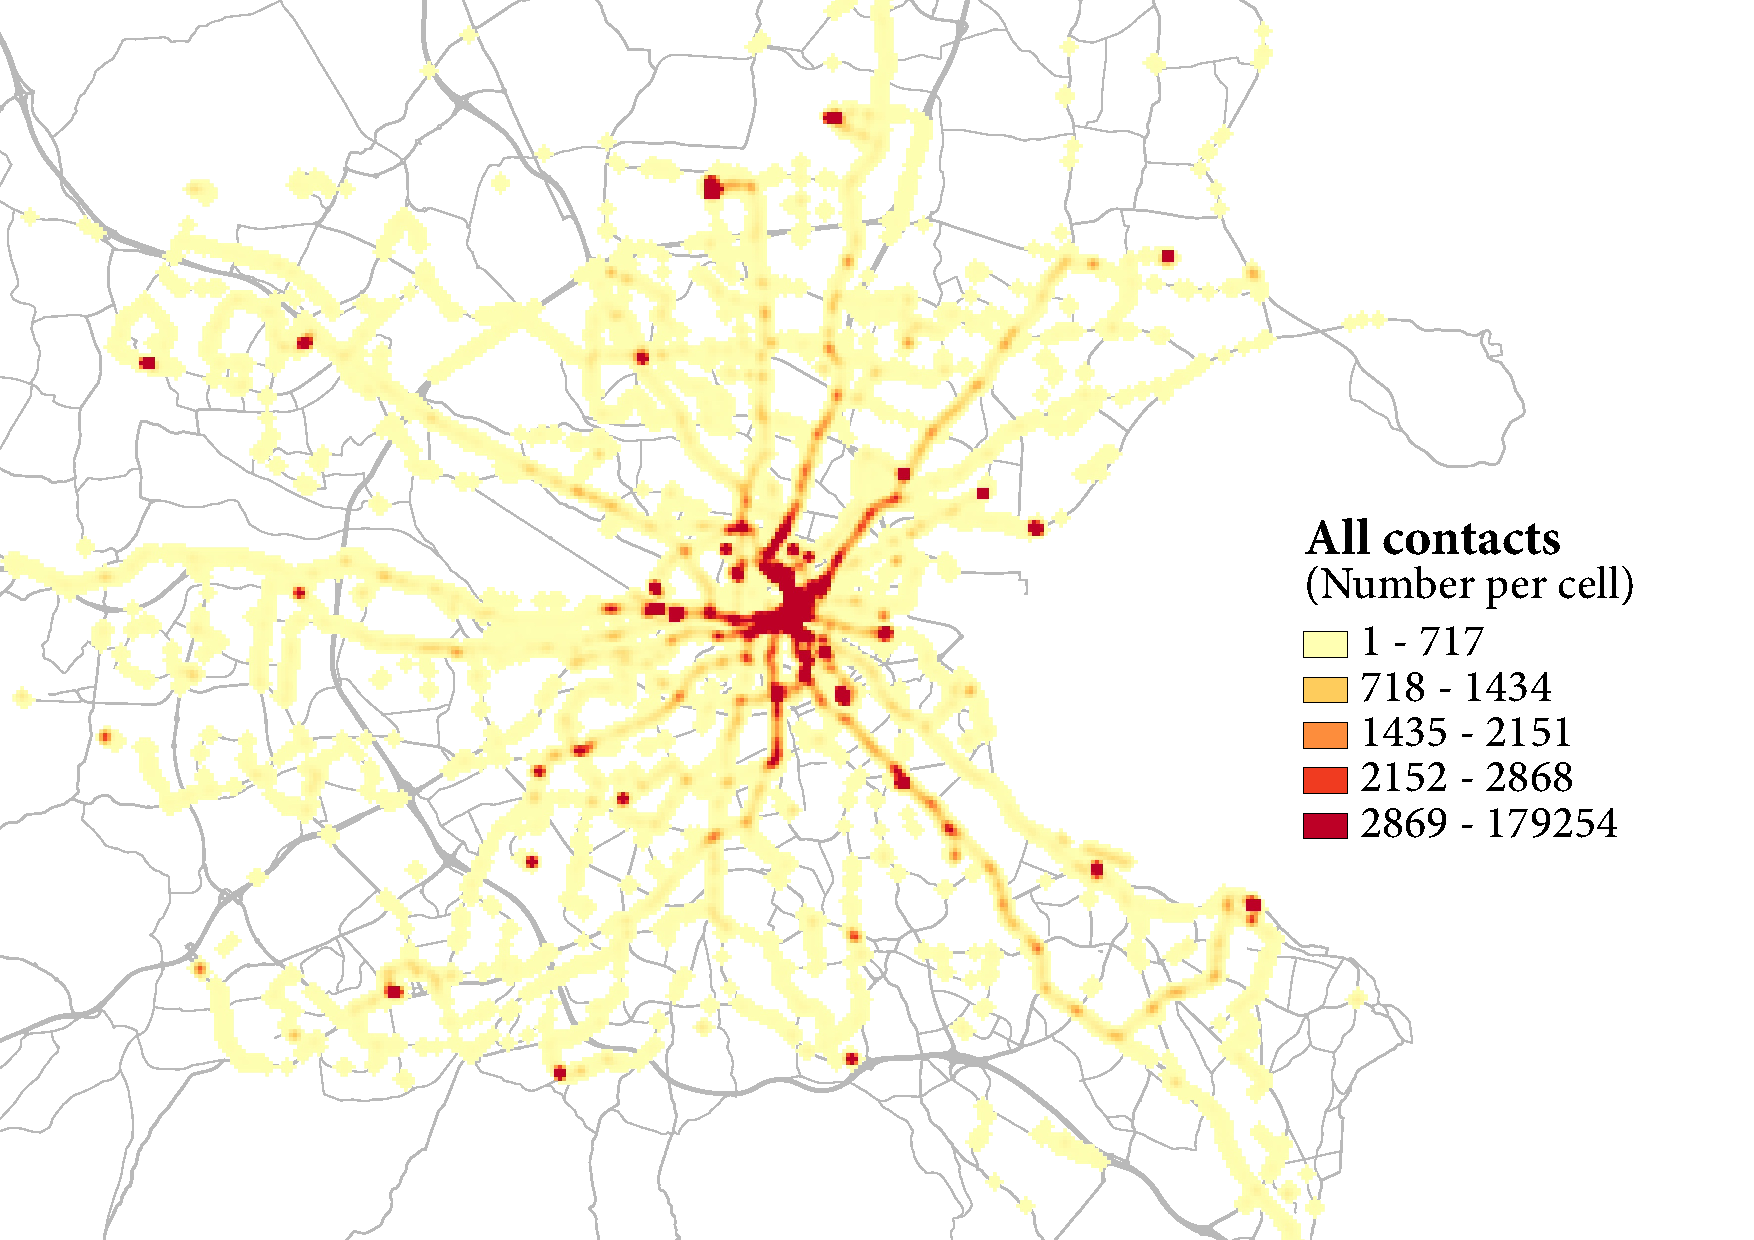
\includegraphics[width=\linewidth]{figures/dublin-all-contacts.pdf}
    \caption{Heatmap of the contacts of any duration in Dublin, Ireland.\vspace{1em}}
    \label{fig:all-contacts}
  \end{subfigure}%
 \qquad
  \begin{subfigure}[t]{.47\textwidth}
    \centering
    \includegraphics[width=\linewidth]{figures/dublin-200-contacts-res.pdf}
    \caption{Heatmap of contacts whose duration is greater than 200 seconds and the hotspots centered at location centered at the aggregated 25~\% densest cells.}
    \label{fig:200-contacts}
  \end{subfigure}
  \caption{Heatmaps of contacts between buses in Dublin, Ireland. The figures denote the number of contacts per cell (of size 100~m $\times$ 100~m). We choose to simulate migrations between buses entering the two hotspots circled on the map of Figure~\ref{fig:200-contacts}.}
  \label{fig:dublin-bus}
\end{figure}


\subsection{Experimentation with a bus system}

In this section, we assess the feasibility of migrating virtual machines in the context of the public transportation system of the city of Dublin.  In our simulations, we focus on the capacity of the opportunistic contacts between buses while in transit.

\paragraph{Experimental setup.} 
For our feasibility study, we use a publicly available dataset of real traces of Dublin city buses provided by Dublinked, part of the Dublin City Council. The mobility traces span the month of January 2013 and provide timestamped GPS coordinates of all DublinBus buses in service~\cite{dublinked}. We analyze the movements of 823 buses during the service day of Tuesday, January 29th, 2013 from 10am to 1pm. We assume that two buses are in contact whenever the buses are in each other's communication radius denoted $R$. We used a recent map-matching algorithm proposed by Newson and Krumm to match the sequence of timestamps positions with the planned route given in the GTFS feed provided by the Dublin City council~\cite{newson2009hidden}. This step allowed us to remove outliers from the simulation, which could bias the results, as well as form more realistic trajectories by adding timestamps waypoints corresponding to the respective routes followed by the buses.

We use the ONE, a discrete-event simulator to run our experiments~\cite{keranen2009one}. The ONE can use real-world mobility traces to reproduce the movements of DTN nodes using linear interpolation between two timestamped waypoints and infer their contacts. We used the default settings of the ONE to simulate IEEE~802.11 on the mobile nodes. However, the only layers supported by the ONE simulator are the network layers and above. To account for the properties of the physical layer including the link-level packet losses, we select appropriate values regarding the node communication radius and contact transfers goodput. We draw on the results presented by Rubinstein \etal which show a 1~Mbps plateau in the TCP goodput when the contact distance between vehicles is less than 150~m~\cite{rubinstein2009measuring}. The choice of a conservative node radius is further supported by Hadaller \etal who showed that the Packet Delivery Ratio (PDR) measured at the MAC layer remain stable between vehicles in contact within a similar distance of 150~m~\cite{hadaller2007vehicular}. In our simulations, we considered a conservative communication radius $R$ of 150~m with a homogeneous average goodput of 1~MB per second. 

\paragraph{VM migration simulations.}
In the remainder of this section, we simulate the migration of virtual machines of various sizes running on every bus. A bus entering a specific hotspot initiates the migration of a virtual machine with the first bus it comes in contact with, following the First Contact routing policy implemented by the ONE simulator. We make no assumption regarding the capacity of the buses to predict the duration of a contact. A transfer will be aborted in case the contact duration is not long enough to accommodate the transfer. Hence, multiple attempts may be needed before the migration succeeds. The migration is considered as failed if the bus exits the hotspot without succeeding in transferring the virtual machine.

The results we present reflect averages over 100~virtual machine migration trials for different sizes of virtual machines we try to migrate at each of the two hotspots introduced in Figure~\ref{fig:200-contacts}. The range of values we use captures the usual sizes of virtual machines that can be found, that is, from a few hundreds of kilobytes (\eg TinyOS~\cite{levis2005tinyos}) to a few hundreds of Megabytes~\cite{clark2005live}. For each size of virtual machine, we measure the average time needed for a bus entering each hotspot to find a suitable contact and the time it actually takes to migrate the virtual machine. The plot in Figure~\ref{fig:graph} shows the mean time to transfer virtual machines of different sizes, as well as the proportion of virtual machines that were actually transferred. 

\begin{figure}[t]
  \centering
  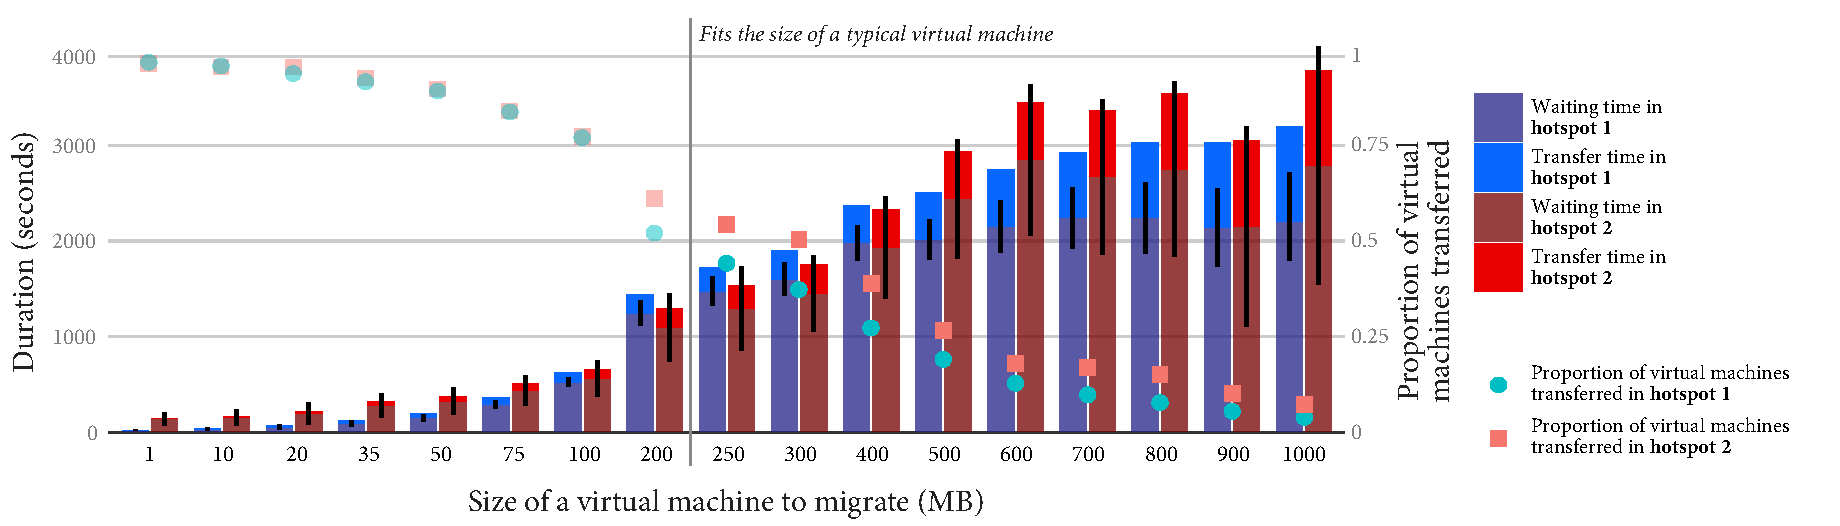
\includegraphics[width=0.98\linewidth]{figures/duration-ratio-migrations.pdf}
  \caption{Proportion of successful virtual machine migrations and mean time to transfer the virtual machine as a function of the virtual machine size. The black solid bars represent the 95\% confidence interval for the waiting time before successfully transferring the virtual machines.}
  \label{fig:graph}
\end{figure} 

\begin{wrapfigure}[12]{o}[0.7\marginparwidth]{8.2cm}
    \vspace{-10pt}
    \centering
    \includegraphics[width=8cm]{figures/contact-durations-histogram.pdf}
    \caption{Number of contacts (in log scale) accounted for different duration ranges and their ratios (in percentage) against the total number of contacts in the hotspots 1 and 2, respectively.}
    \label{fig:plot-contact-duration-ratio}
%\end{figure}
\end{wrapfigure}
First, we note that the ratio of virtual machines successfully migrated at both hotspots decreases as their size increases. This is due to the lack of enough long-lasting contacts between buses. Buses fail several times before finding a suitable contact to transfer the virtual machine. This observation is confirmed by the time spent waiting for a contact suitable in duration with large-sized virtual machines. Overall, it takes less time to find a suitable contact at hotspot~1 than at hotspot~2. Buses entering hotspot~1 spend less time waiting for a suitable contact in comparison with hotspot~2 expect for virtual machine sizes ranging from 200 to 400~MB. To further explain this trend, we plot in~Figure~\ref{fig:plot-contact-duration-ratio} the total number of contacts measured for different contact durations as well as the ratios of those contacts against the total number of contacts occurring in  hotspots~1 and~2. We can see that hotspot~2 has a higher ratio of contacts lasting long enough (\eg 200~s and 400~s) to accommodate transfers of virtual machines with a size ranging from 200~MB to 400~MB. Despite the higher number of contacts at hotspot~1, most of them are not suitable for the transfers of such virtual machines. Buses spent more time trying transfers that will eventually fail before finding a suitable contact. This also explains why the ratio of successful migrations is higher at hotspot~2 when virtual machines have sizes ranging from 200 to 400~MB.


\section{Discussions}

\paragraph{Atomic contacts (first extension).}
The stronger assumption we made is to consider contacts between mobile users and repositories with unlimited capacity. If we want to relax this assumption, an increasing number of requests would not be satisfied with the simulation time. We need to consider the following enablers. Firstly, with equal file size and control messages with negligible size, we have to adapt the placement algorithm to take the contact duration of buses at each candidate repository. In particular, we need to differentiate the (longer) contacts of buses with repositories located in bus stops where the buses will actually stop at, and the (shorter) contacts between buses and repositories located in bus stops where the bus does not stop at. Secondly, we need to prioritize the requests to transfer between the repository and the bus. As an example, the \texttt{put} requests must be transmitted to the repository before any other request. Similarly, if the repository can satisfy the \texttt{get} requests carried by the bus, the corresponding files must be transmitted before the files associated with the \texttt{sync} requests of the bus and the repository. Finally, we note the different priorities impacts the replication of the data across the repositories. As a result, we need to develop new strategies to decrease the number of copies to replicate. 

\begin{wrapfigure}[14]{o}[0.7\marginparwidth]{6.7cm}
    \vspace{-15pt}
    \centering
    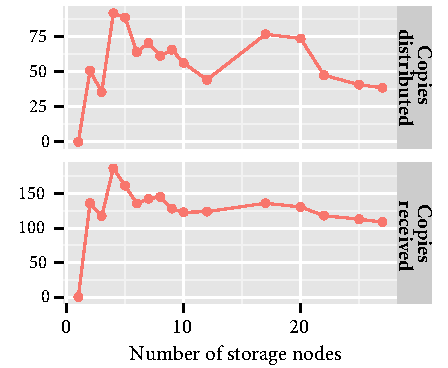
\includegraphics[width=6.5cm]{figures/allput-backend.pdf}
    \caption{Average number of copies distributed and received by the repositories for a file and a user request deadline of 2400~seconds.}
    \label{fig:allput-backend}
%\end{figure}
\end{wrapfigure}
\paragraph{Replication strategies (first extension).}
With the replication of file copies to every repository, a large number of copies is distributed and received by the repositories, as we show in Figure~\ref{fig:allput-backend}. With non-atomic contacts, we need to limit the overhead of copies sent over contacts between mobile users and repositories. With no knowledge of the future trajectories of mobile users, one could distribute copies of files for a bounded duration until the distribution of copies of the file stops. Alternatively, one could bound the number of copies generated per repository and transmitted to the mobiles users. With techniques borrowed from Delay Tolerant Networks, one could use a control plane that would enable the repositories to ``learn'' the frequent repositories the mobile users encounter along their route~\cite{lindgren2003probabilistic,grossglauser2006locating}. With this information, a single copy would be needed to transmit per repository. 

\paragraph{Virtual machine allocation (second extension).}
Recall that we considered a set of virtual machines managed by an infrastructure provider who allocates them to service providers who deploy their services. However, we did not detail the algorithm to allocate the virtual machines to the service providers such that the allocation result satisfies their requirements. As an example, the requirements may relate to the number of virtual machines to allocate, a target guaranteed connectivity of virtual machines through vehicle-to-vehicle connectivity, or the geographic areas covered by the virtual machines. The output of the allocation algorithm must minimize the number of migrations and where they happen in order to minimize the duration of the transition. Additionally, the service providers may issue new demands to the infrastructure provider or change their current demands. To this end, the latter must determine whether the demands can be satisfied before serving them. An approach to achieve this is to check the current state of the available and allocated resources through the control channel before allocating new resources. If the demand can be allocated or modified, the infrastructure provider re-runs an allocation algorithm that triggers new slicing of the resources of the nodes, as well as virtual machine migration between the mobile nodes.

\paragraph{Finding suitable contacts (second extension).} In order to successfully transfer a virtual machine between two vehicles, the contact must be long enough to accommodate the size of the virtual machine. In our evaluation, we proposed a methodology to determine the geographical areas we refer to as hotspots where long-duration contacts occur at significant rates. Hotspots are located in geographical areas within which all contacts amount for 75\% of all 200~second long contacts and occur at most every 1000~seconds. However, although long-duration contacts occur statistically more often in the hotspots compared to other areas, there is still a high density of short-duration contacts (as shown in Figure~\ref{fig:200-contacts}). Depending on the first contact a bus has when entering a hotspot, the VM migration may fail if the first contact is not long enough to accommodate the target virtual machine size. One way of improving the migration success is tu use models to predict contact durations between buses. Many existing techniques may be borrowed from the DTN literature. For instance, this could be done by maintaining a list of contact with their corresponding durations for each vehicle encountered~\cite{lindgren2003probabilistic,grossglauser2006locating} or by exchanging the direction and speed or itinerary between vehicles in contact to estimate the shared route with the other vehicle~\cite{cheng2010geodtn,banerjee2007energy}.

\section{Conclusion}

In this chapter, we proposed to extend the concept of offloading spots into two distinct directions in the context of different vehicular cloud services. In both extensions, we relied on a logical map to characterize the movements of the vehicles within the offloading spots or between them. We then used this logical map to determine the placement of the offloading spot to optimize the resulting compositions of the movements of the vehicles according to the service requirements.

In the first extension, we proposed a placement of offloading spots that act as repositories that are part of a distributed cloud-like storage and sharing system. The placement aims to satisfy a maximum of user requests to store or retrieve files and distribute the files throughout the repository network using the movements of the mobile users between the repositories. We showed the benefits of using the movements of vehicles to distribute files and thus improve the success ratio of the user requests.

In the second extension, we dematerialized offloading spots into pre-defined areas where vehicle often meet long enough to transfer large amounts of data. We used these areas in the context of a virtualization of the resources of the vehicles to migrate virtual machines following topology changes. We proposed a placement of these areas such that the vehicles can accommodate large data transfers of the size of a virtual machine. With simulations of real-world bus traces, we showed that these areas increase the success of the transfers as the vehicles are more likely to come in contact with other vehicles for long durations. As a result, transfers of several hundreds of Megabytes can be achieved through \acrshort{v2v} communications, enough to accommodate migrations of virtual machines.

These extensions showed that the existing mobility of vehicles has the potential to provide innovative added-value services for urban environments, with limited reliance on conventional data networks.